\section{Actividad 4: k-d tree para clasificación 1-NN}
\label{sec:act4}


En esta actividad implementamos un k-d tree, construido con Dividir para Conquistar, y
lo usamos para clasificar dígitos manuscritos con 1-NN. Comparamos su búsqueda exacta del
vecino más cercano con la búsqueda exhaustiva para distintas dimensionalidades,
obtenidas con PCA, y observamos cómo esa reducción afecta la clasificación.

El código está en el repositorio: \texttt{src/kdtree.py} tiene la estructura y las dos
búsquedas, y \texttt{scripts/act4\_kdtree.py} ejecuta los experimentos y genera las
tablas y figuras de esta sección, con el comando \texttt{python scripts/act4\_kdtree.py}.

% ============================================================
\subsection{Implementación}

\textbf{Distancia.} Las dos estrategias usan la misma función para la distancia euclidiana
al cuadrado, escrita con el mismo ciclo del enunciado:
\begin{lstlisting}
def squared_distance(a, b):
    suma = 0.0
    for j in range(len(a)):
        diff = a[j] - b[j]
        suma = suma + diff * diff
    return suma
\end{lstlisting}

\textbf{Estructura.} Cada nodo es un diccionario que guarda un punto, su posición en el
conjunto de entrenamiento, el eje de partición y referencias a sus dos hijos.

\textbf{Construcción.} Es la aplicación de Dividir para Conquistar de esta actividad. En
cada llamada se elige el eje como \texttt{depth mod d}, se ordenan los puntos según ese
eje, se toma la mediana $m = \floor{n/2}$ como nodo y se construyen recursivamente los dos
subárboles, con los puntos a la izquierda y a la derecha de la mediana. Es el algoritmo de
la Actividad 3.2, así que la construcción cuesta $\T{n\log^2 n}$. Como la mediana divide
los puntos en dos mitades, el árbol queda balanceado y tiene altura
$\floor{\log_2 n} + 1$. Con los $1437$ puntos de entrenamiento, eso son $11$ niveles.

\textbf{Búsqueda exacta.} Sigue el esquema del enunciado:
\begin{lstlisting}
def buscar(nodo, q, mejor):
    # `mejor` guarda el mejor vecino encontrado y los nodos visitados.
    if nodo is None:
        return

    mejor["visitados"] = mejor["visitados"] + 1
    dist = squared_distance(q, nodo["punto"])
    if dist < mejor["dist"]:
        mejor["dist"] = dist
        mejor["indice"] = nodo["indice"]

    eje = nodo["eje"]
    delta = q[eje] - nodo["punto"][eje]
    if delta < 0:
        cerca = nodo["izquierdo"]
        lejos = nodo["derecho"]
    else:
        cerca = nodo["derecho"]
        lejos = nodo["izquierdo"]

    buscar(cerca, q, mejor)
    if delta * delta < mejor["dist"]:
        buscar(lejos, q, mejor)
\end{lstlisting}
Primero se visita el subárbol del lado de la consulta. El otro se explora solo si
$\delta^2$, la distancia al cuadrado de la consulta al hiperplano de corte, es menor que
la mejor distancia encontrada. Esa prueba se hace después de explorar el lado cercano,
porque ahí la mejor distancia puede haber bajado. La poda no pierde el vecino exacto:
todos los puntos del otro lado están al menos a distancia $|\delta|$ de la consulta, así
que si $\delta^2$ ya no es menor que la mejor distancia, ninguno de ellos puede mejorarla.
Cada nodo visitado evalúa exactamente una distancia, así que el número de nodos visitados
es también el número de distancias evaluadas.

\textbf{Búsqueda exhaustiva.} Recorre los $n_{\text{train}}$ puntos y se queda con el de
menor distancia, así que evalúa exactamente $n_{\text{train}}$ distancias por consulta.

\textbf{Comparación justa.} Las dos búsquedas están escritas en Python puro, trabajan
sobre los mismos datos (listas de números) y usan la misma \texttt{squared\_distance}. No
se usa NumPy ni ninguna operación vectorizada en ninguna de las dos. Así, la diferencia de
tiempo refleja principalmente cuántas distancias evalúa cada estrategia.

% ============================================================
\subsection{Protocolo experimental}

Usamos el conjunto \texttt{digits} de scikit-learn: $1797$ imágenes de $8 \times 8$
píxeles, con $64$ características y etiquetas de $0$ a $9$. Los datos se separan en
80\,\% entrenamiento ($1437$ imágenes) y 20\,\% prueba ($360$ imágenes), de forma
estratificada y con \texttt{random\_state=42}. Las características se estandarizan con la
media y la desviación del conjunto de entrenamiento, y luego se aplica PCA, ajustado
también solo con entrenamiento, para obtener $d \in \{2, 4, 8, 16, 32\}$ componentes.
scikit-learn se usa únicamente para estos pasos y para la accuracy.

Para cada $d$ se construye el k-d tree sobre los datos de entrenamiento y se clasifican las
$360$ imágenes de prueba con las dos búsquedas. Cada tiempo es la mediana de $7$
repeticiones, y no incluye la carga de datos, la estandarización ni PCA. Como referencia,
agregamos una fila con las $64$ componentes (marcada con $^{*}$), que tiene la misma
geometría que los datos sin reducir. Los experimentos se ejecutaron en un computador con
procesador Apple M2, Python 3.12.2 y scikit-learn 1.6.1.

% ============================================================
\subsection{Correctitud y accuracy}

\begin{table}[H]
  \centering
  \caption{Validación del k-d tree con la búsqueda exhaustiva como referencia, y accuracy
  1-NN en el conjunto de prueba.}
  \small
  \begin{tabular}{crrrr}
\toprule
$d$ & accuracy exhaustiva & accuracy k-d tree & misma distancia mínima & mismo vecino \\
\midrule
2 & 0{,}4472 & 0{,}4472 & 100{,}0\,\% & 100{,}0\,\% \\
4 & 0{,}8056 & 0{,}8056 & 100{,}0\,\% & 100{,}0\,\% \\
8 & 0{,}9306 & 0{,}9306 & 100{,}0\,\% & 100{,}0\,\% \\
16 & 0{,}9583 & 0{,}9583 & 100{,}0\,\% & 100{,}0\,\% \\
32 & 0{,}9722 & 0{,}9722 & 100{,}0\,\% & 100{,}0\,\% \\
64$^{*}$ & 0{,}9667 & 0{,}9667 & 100{,}0\,\% & 100{,}0\,\% \\
\bottomrule
\end{tabular}

\end{table}

Para todas las dimensiones, el k-d tree encuentra la misma distancia mínima y el mismo
vecino que la búsqueda exhaustiva en el 100\,\% de las consultas. No hubo empates, así
que el vecino también coincide siempre. Por eso las dos estrategias tienen exactamente la
misma accuracy.

% ============================================================
\subsection{Resultados}

\begin{table}[H]
  \centering
  \caption{Tiempos (mediana de 7 repeticiones) y speedup de consulta
  $S = T_{\text{exhaustiva}} / T_{\text{k-d tree}}$.}
  \resizebox{\linewidth}{!}{\begin{tabular}{crrrrrr}
\toprule
$d$ & construcción (ms) & exhaustiva total (s) & exhaustiva / consulta (ms) & k-d tree total (s) & k-d tree / consulta (ms) & speedup $S$ \\
\midrule
2 & 4{,}6 & 0{,}085 & 0{,}237 & 0{,}002 & 0{,}006 & 38{,}85 \\
4 & 2{,}7 & 0{,}115 & 0{,}320 & 0{,}008 & 0{,}022 & 14{,}57 \\
8 & 2{,}4 & 0{,}175 & 0{,}487 & 0{,}039 & 0{,}109 & 4{,}46 \\
16 & 3{,}3 & 0{,}285 & 0{,}792 & 0{,}133 & 0{,}368 & 2{,}15 \\
32 & 2{,}4 & 0{,}559 & 1{,}552 & 0{,}313 & 0{,}868 & 1{,}79 \\
64$^{*}$ & 2{,}4 & 1{,}001 & 2{,}781 & 0{,}735 & 2{,}041 & 1{,}36 \\
\bottomrule
\end{tabular}
}
\end{table}

\begin{table}[H]
  \centering
  \caption{Trabajo por consulta: nodos visitados por el k-d tree, fracción del conjunto de
  entrenamiento ($n_{\text{train}} = 1437$) y distancias evaluadas en total por cada
  método para las $360$ consultas.}
  \resizebox{\linewidth}{!}{\begin{tabular}{crrrrrr}
\toprule
$d$ & visitados (promedio) & visitados (mediana) & fracción visitada & $1/\text{fracción}$ & distancias exhaustiva & distancias k-d tree \\
\midrule
2 & 17{,}2 & 16 & 0{,}012 & 83{,}5 & 517\,320 & 6\,199 \\
4 & 53{,}8 & 45 & 0{,}037 & 26{,}7 & 517\,320 & 19\,372 \\
8 & 209{,}2 & 158 & 0{,}146 & 6{,}9 & 517\,320 & 75\,296 \\
16 & 492{,}3 & 373 & 0{,}343 & 2{,}9 & 517\,320 & 177\,239 \\
32 & 737{,}4 & 656 & 0{,}513 & 1{,}9 & 517\,320 & 265\,475 \\
64$^{*}$ & 955{,}5 & 891 & 0{,}665 & 1{,}5 & 517\,320 & 343\,970 \\
\bottomrule
\end{tabular}
}
\end{table}

\begin{figure}[H]
  \centering
  \begin{subfigure}{0.49\linewidth}
    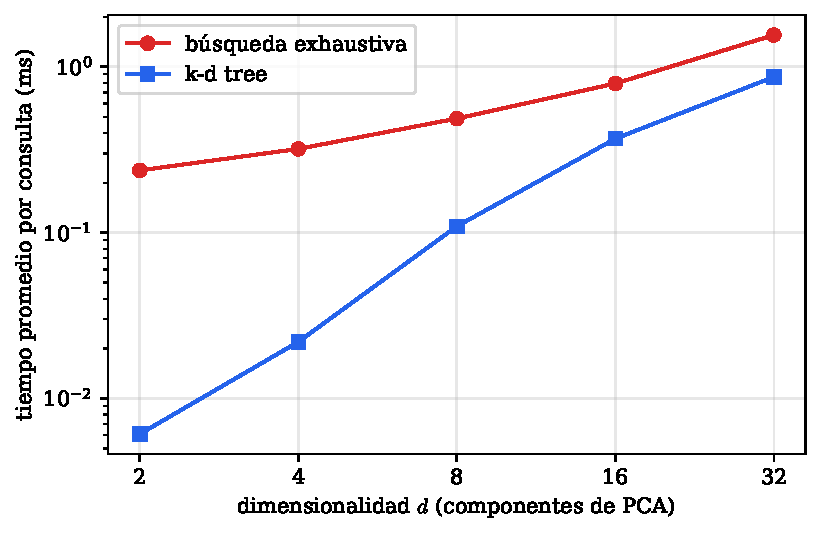
\includegraphics[width=\linewidth]{act4_tiempo_consulta.pdf}
    \caption{Tiempo promedio por consulta.}
  \end{subfigure}\hfill
  \begin{subfigure}{0.49\linewidth}
    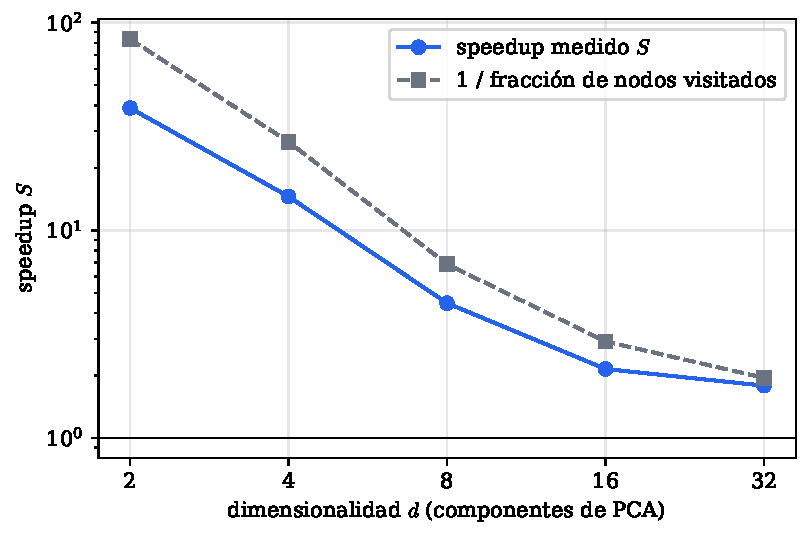
\includegraphics[width=\linewidth]{act4_speedup.pdf}
    \caption{Speedup y $1/\text{fracción visitada}$.}
  \end{subfigure}

  \medskip
  \begin{subfigure}{0.49\linewidth}
    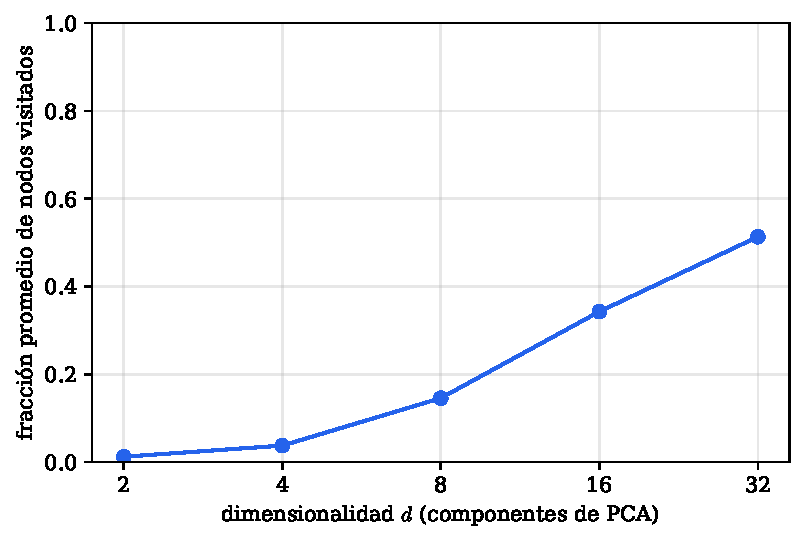
\includegraphics[width=\linewidth]{act4_fraccion_visitada.pdf}
    \caption{Fracción promedio de nodos visitados.}
  \end{subfigure}\hfill
  \begin{subfigure}{0.49\linewidth}
    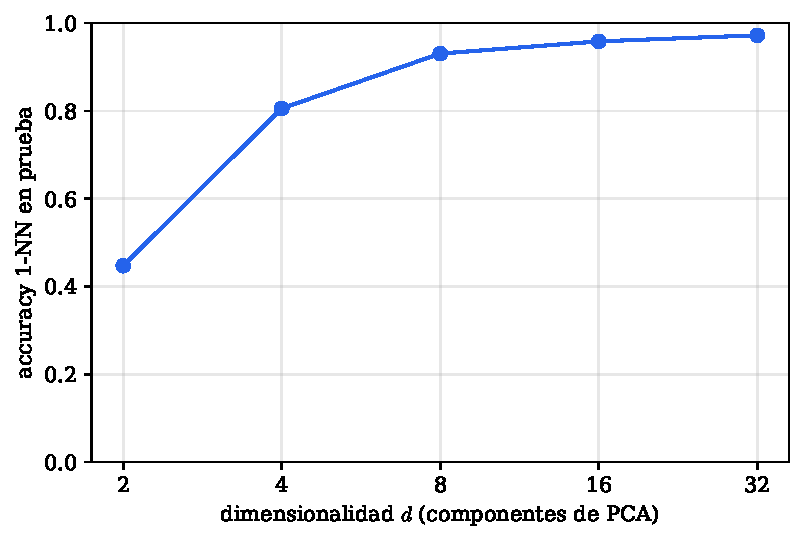
\includegraphics[width=\linewidth]{act4_accuracy.pdf}
    \caption{Accuracy 1-NN.}
  \end{subfigure}
  \caption{Resultados en función de la dimensionalidad $d$. Los ejes horizontales están en
  escala logarítmica, y los verticales de (a) y (b) también.}
\end{figure}

\begin{figure}[H]
  \centering
  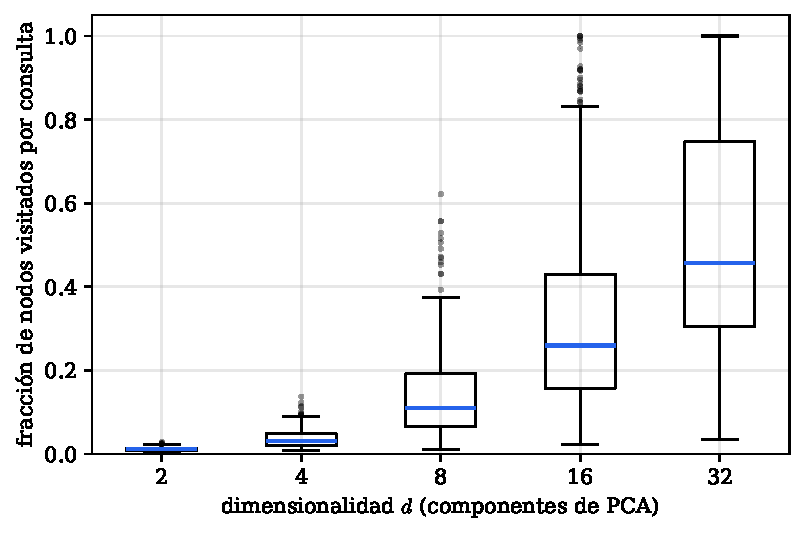
\includegraphics[width=0.7\linewidth]{act4_visitados_distribucion.pdf}
  \caption{Distribución de la fracción de nodos visitados por consulta. Cada caja va del
  primer al tercer cuartil y la línea interior es la mediana.}
\end{figure}

El tiempo de construcción es de unos pocos milisegundos y casi no cambia con $d$, porque
el ordenamiento en cada llamada compara una sola coordenada, sin importar cuántas tenga
cada punto. Con la búsqueda exhaustiva, en cambio, el tiempo por consulta crece con $d$,
porque cada una de las $1437$ distancias recorre $d$ coordenadas.

% ============================================================
\subsection{Discusión}

\textbf{(a) ¿Para qué valores de $d$ el k-d tree reduce claramente el trabajo y el
tiempo?} Para $d = 2$ y $d = 4$ la reducción es grande: el árbol visita cerca del 1\,\% y
del 4\,\% de los puntos, y es unas $39$ y $15$ veces más rápido que la búsqueda
exhaustiva. Con $d = 8$ la ganancia sigue siendo clara: visita cerca del 15\,\% y es unas
$4{,}5$ veces más rápido. Desde $d = 16$ la ganancia es pequeña, de cerca de $2$ veces, y
con $d = 32$ baja a $1{,}8$.

El speedup sigue de cerca al inverso de la fracción de nodos visitados, como se ve en el
gráfico (b). Esto es lo esperable, porque las dos estrategias pagan lo mismo por cada
distancia: si el árbol evalúa la décima parte de las distancias, debería tardar cerca de
la décima parte. El speedup queda algo por debajo de ese valor porque cada nodo visitado
tiene un costo extra que la búsqueda exhaustiva no tiene: la llamada recursiva, el cálculo
de $\delta$ y la decisión de qué lado explorar. Ese costo extra pesa más cuando $d$ es
pequeño, porque ahí una distancia es barata de calcular. Con $d = 2$ el árbol evalúa unas
$83$ veces menos distancias, pero es unas $39$ veces más rápido.

\textbf{(b) ¿Qué ocurre con la fracción de nodos visitados cuando aumenta $d$?} Crece de
forma sostenida: cerca de 1\,\%, 4\,\%, 15\,\%, 34\,\% y 51\,\% para
$d = 2, 4, 8, 16$ y $32$, y llega a 66\,\% con las $64$ componentes. Con más dimensiones,
la distancia de la consulta a cada hiperplano de corte, que mide una sola coordenada, es
pequeña comparada con la distancia al mejor vecino, que suma las diferencias en todas las
coordenadas. Por eso la condición $\delta^2 <$ \texttt{bestDist} se cumple más seguido y
hay que revisar más subárboles. Además, el árbol tiene solo $11$ niveles, así que con
$d = 16$ o $d = 32$ cada camino de la raíz a una hoja corta por a lo más $11$ coordenadas
distintas, y el resto nunca se usa para descartar regiones.

\textbf{(c) ¿Son consistentes los resultados con un peor caso $\Theta(n)$?} Sí. Con
$d = 16$ y $d = 32$ hay consultas que visitan los $1437$ nodos del árbol, es decir, que
hacen el mismo trabajo que la búsqueda exhaustiva, y con $d = 32$ la mediana de nodos
visitados ya es casi la mitad del conjunto. La búsqueda es exacta, y cuando la poda no
logra descartar regiones, termina revisando todos los puntos. El k-d tree no garantiza un
costo logarítmico por consulta: su ventaja depende de la dimensionalidad y de cómo están
distribuidos los datos.

\textbf{(d) ¿Hay relación entre reducir la dimensión con PCA y la accuracy?} Sí. La
accuracy sube de cerca de $0{,}45$ con $d = 2$ a $0{,}81$ con $d = 4$, $0{,}93$ con
$d = 8$, $0{,}96$ con $d = 16$ y $0{,}97$ con $d = 32$. Con pocas componentes se pierde
información que distingue unos dígitos de otros, y el vecino más cercano en ese espacio
reducido muchas veces es de otra clase. Con las $64$ componentes la accuracy es levemente
menor que con $32$, así que más dimensiones no siempre ayudan: las últimas componentes
aportan poca información y algo de ruido.

Esta variación viene de la representación de los datos y no de la búsqueda. Para cada $d$,
el k-d tree y la búsqueda exhaustiva encuentran el mismo vecino en todas las consultas, y
por eso tienen exactamente la misma accuracy. Lo que cambia al variar $d$ es el espacio en
que se miden las distancias, y con él cuál es el vecino más cercano. Esto deja un
compromiso: reducir la dimensión acelera mucho el k-d tree, pero empeora la
clasificación. En este conjunto, $d = 8$ parece un buen punto intermedio, con una accuracy
de $0{,}93$ y una búsqueda unas $4{,}5$ veces más rápida.

\textbf{(e) ¿Por qué el análisis asintótico y la medición experimental se complementan?}
El análisis asintótico describe cómo crece el costo con $n$ y da garantías para cualquier
entrada: la construcción es $\T{n\log^2 n}$ y una consulta exacta puede costar $\T{n}$ en
el peor caso. Pero oculta las constantes y no dice cuánto se poda con unos datos
concretos. La medición muestra el costo real con estos datos, este $n$ y este computador,
incluido el costo extra de la recursión, y permite ver que el caso típico está muy lejos
del peor caso cuando $d$ es pequeño. A su vez, la medición sola no permite generalizar a
otros tamaños o conjuntos de datos, y sus tiempos dependen del hardware. Por eso ninguna
de las dos reemplaza a la otra.

